% !TEX root = ../main.tex
% !TEX root = ../main.tex
% Measurement setups (I-U, P-I, spectral), redrawn in TikZ.
% Include with % !TEX root = ../main.tex
% Measurement setups (I-U, P-I, spectral), redrawn in TikZ.
% Include with % !TEX root = ../main.tex
% Measurement setups (I-U, P-I, spectral), redrawn in TikZ.
% Include with \input{chapters/measurement_setup.tex}; reference the whole figure
% with \cref{fig:setup} or a single setup with \cref{fig:setup_iu},
% \cref{fig:setup_pi} and \cref{fig:setup_spectral}.

\tikzset{
	setup/.style={font=\small, line width=0.6pt},
	meter/.style={circle, draw, fill=white, minimum size=0.75cm, inner sep=0pt},
	% instrument box with display; terminals (-a) left and (-b) right, origin at (-b)
	instrument/.pic={
		\draw (-2.8,-0.35) rectangle (0.25,1.0);
		\node[draw, rounded corners=2pt, anchor=north west, minimum width=1.2cm,
			minimum height=0.4cm, inner sep=2pt] at (-2.65,0.85) {#1};
		\fill (-0.25,0) circle (2pt) coordinate (-a);
		\fill (0,0) circle (2pt) coordinate (-b);
	},
	ground/.pic={
		\draw (0,0) -- (0,-0.9);
		\draw[line width=1.4pt] (-0.3,-0.9) -- (0.3,-0.9);
	},
	% laser diode pointing to the right, centred at the origin
	diode/.pic={
		\fill (-0.18,0.2) -- (-0.18,-0.2) -- (0.18,0) -- cycle;
		\draw[line width=1.2pt] (0.18,0.2) -- (0.18,-0.2);
	},
	emission/.pic={
		\draw[-{Stealth[length=4pt]}] (-0.15,0.3) -- (0.2,0.7);
		\draw[-{Stealth[length=4pt]}] (0.05,0.3) -- (0.4,0.7);
	},
	% temperature-controlled mount below the diode
	mount/.pic={
		\draw[fill=gray!30] (-0.12,-0.25) rectangle (0.12,-1.0);
		\draw[fill=gray!60] (-0.3,-1.0) rectangle (0.3,-1.15);
	},
}

\begin{figure}[H]
	\centering
	\begin{subfigure}{\linewidth}
		\centering
		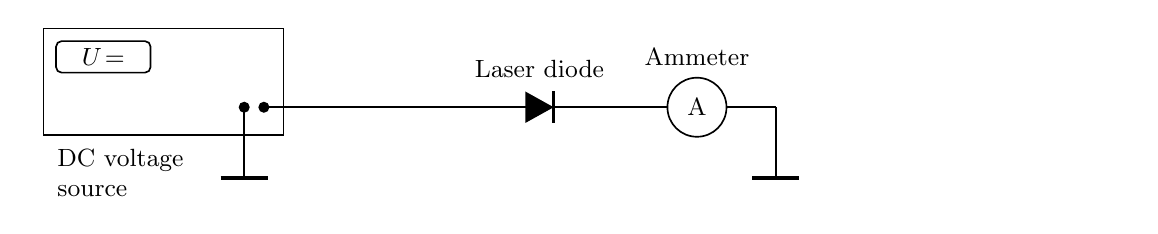
\begin{tikzpicture}[setup]
			\path (-3,0) -- (11,0);
			\pic (src) at (0,0) {instrument={$U\!=$}};
			\node[anchor=north west, align=left] at (-2.75,-0.4) {DC voltage\\source};
			\pic at (src-a) {ground};
			\draw (src-b) -- (6.5,0);
			\pic at (3.5,0) {diode};
			\node[above] at (3.5,0.25) {Laser diode};
			\node[meter] at (5.5,0) {A};
			\node[above] at (5.5,0.4) {Ammeter};
			\pic at (6.5,0) {ground};
		\end{tikzpicture}
		\caption{Current-voltage characteristic.}
		\label{fig:setup_iu}
	\end{subfigure}

	\vspace{0.6cm}
	\begin{subfigure}{\linewidth}
		\centering
		\begin{tikzpicture}[setup]
			\path (-3,0) -- (11,0);
			\pic (gen) at (0,0) {instrument={$I\!=$}};
			\node[anchor=north west, align=left] at (-2.75,-0.4) {Pulse\\generator};
			\pic at (gen-a) {ground};
			\draw (gen-b) -- (5.9,0);
			\draw (0.6,0.15) -- (0.9,0.15) -- (0.9,0.6) -- (1.2,0.6) -- (1.2,0.15) -- (1.5,0.15);
			% voltage measurement at the diode
			\fill (2.2,0) circle (2pt);
			\node[meter] (V) at (2.2,-1.0) {U};
			\draw (2.2,0) -- (V);
			\pic at (V.south) {ground};
			% laser diode on mount with detector
			\pic at (3.6,0) {mount};
			\pic at (3.6,0) {diode};
			\pic at (3.6,0) {emission};
			\draw (4.3,0.8) rectangle (5.5,1.1);
			\node[above] at (4.9,1.1) {Detector};
			\node[meter] at (5.1,0) {A};
			\pic at (5.9,0) {ground};
			% lock-in amplifier
			\pic (lock) at (10.5,0) {instrument={Lock-in}};
			\draw (5.5,0.95) -- (6.8,0.95) -- (6.8,-0.6) -- (10.25,-0.6) -- (lock-a);
			\pic at (lock-b) {ground};
		\end{tikzpicture}
		\caption{Optical power-current characteristic.}
		\label{fig:setup_pi}
	\end{subfigure}

	\vspace{0.6cm}
	\begin{subfigure}{\linewidth}
		\centering
		\begin{tikzpicture}[setup]
			\path (-3,0) -- (11,0);
			\pic (src) at (0,0) {instrument={$I\!=$}};
			\node[anchor=north west, align=left] at (-2.75,-0.4) {DC current\\source};
			\pic at (src-a) {ground};
			\draw (src-b) -- (5.3,0);
			\pic at (3.2,0) {mount};
			\pic at (3.2,0) {diode};
			\pic at (3.2,0) {emission};
			\node[meter] at (4.5,0) {A};
			\pic at (5.3,0) {ground};
			% lens focusing onto the monochromator entrance slit
			\draw (4.0,1.25) ellipse (0.12 and 0.42);
			\draw (4.1,1.6) -- (6.0,1.25) -- (4.1,0.9);
			\draw (6.0,0.6) rectangle (9.2,1.9);
			\node[anchor=south east] at (9.2,0.6) {Monochromator};
			\draw (9.2,1.3) rectangle (10.3,1.9);
			\node at (9.75,1.6) {PMT};
			% computer
			\draw[rounded corners=2pt] (7.9,-1.05) rectangle (9.1,0.05);
			\draw[rounded corners=1pt] (8.05,-0.9) rectangle (8.95,-0.1);
			\draw (8.3,-1.05) -- (8.2,-1.3) -- (8.8,-1.3) -- (8.7,-1.05);
			\draw (7.6,-1.3) rectangle (9.6,-1.85);
			\foreach \x in {7.75,7.85,...,8.45} \draw (\x,-1.42) -- (\x,-1.73);
			\draw (8.9,-1.5) rectangle (9.4,-1.65);
			\draw (9.75,1.3) .. controls (9.9,0.0) and (10.1,-1.4) .. (9.6,-1.55);
		\end{tikzpicture}
		\caption{Spectral measurements.}
		\label{fig:setup_spectral}
	\end{subfigure}
	\caption{Measurement setups for the characterisation of the laser diode. The diode
	is placed on a temperature-controlled mount for the P-I and spectral measurements.
	PMT: photomultiplier tube.}
	\label{fig:setup}
\end{figure}
; reference the whole figure
% with \cref{fig:setup} or a single setup with \cref{fig:setup_iu},
% \cref{fig:setup_pi} and \cref{fig:setup_spectral}.

\tikzset{
	setup/.style={font=\small, line width=0.6pt},
	meter/.style={circle, draw, fill=white, minimum size=0.75cm, inner sep=0pt},
	% instrument box with display; terminals (-a) left and (-b) right, origin at (-b)
	instrument/.pic={
		\draw (-2.8,-0.35) rectangle (0.25,1.0);
		\node[draw, rounded corners=2pt, anchor=north west, minimum width=1.2cm,
			minimum height=0.4cm, inner sep=2pt] at (-2.65,0.85) {#1};
		\fill (-0.25,0) circle (2pt) coordinate (-a);
		\fill (0,0) circle (2pt) coordinate (-b);
	},
	ground/.pic={
		\draw (0,0) -- (0,-0.9);
		\draw[line width=1.4pt] (-0.3,-0.9) -- (0.3,-0.9);
	},
	% laser diode pointing to the right, centred at the origin
	diode/.pic={
		\fill (-0.18,0.2) -- (-0.18,-0.2) -- (0.18,0) -- cycle;
		\draw[line width=1.2pt] (0.18,0.2) -- (0.18,-0.2);
	},
	emission/.pic={
		\draw[-{Stealth[length=4pt]}] (-0.15,0.3) -- (0.2,0.7);
		\draw[-{Stealth[length=4pt]}] (0.05,0.3) -- (0.4,0.7);
	},
	% temperature-controlled mount below the diode
	mount/.pic={
		\draw[fill=gray!30] (-0.12,-0.25) rectangle (0.12,-1.0);
		\draw[fill=gray!60] (-0.3,-1.0) rectangle (0.3,-1.15);
	},
}

\begin{figure}[H]
	\centering
	\begin{subfigure}{\linewidth}
		\centering
		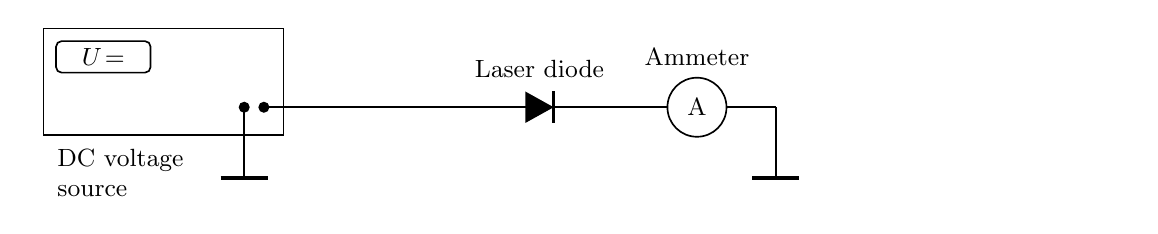
\begin{tikzpicture}[setup]
			\path (-3,0) -- (11,0);
			\pic (src) at (0,0) {instrument={$U\!=$}};
			\node[anchor=north west, align=left] at (-2.75,-0.4) {DC voltage\\source};
			\pic at (src-a) {ground};
			\draw (src-b) -- (6.5,0);
			\pic at (3.5,0) {diode};
			\node[above] at (3.5,0.25) {Laser diode};
			\node[meter] at (5.5,0) {A};
			\node[above] at (5.5,0.4) {Ammeter};
			\pic at (6.5,0) {ground};
		\end{tikzpicture}
		\caption{Current-voltage characteristic.}
		\label{fig:setup_iu}
	\end{subfigure}

	\vspace{0.6cm}
	\begin{subfigure}{\linewidth}
		\centering
		\begin{tikzpicture}[setup]
			\path (-3,0) -- (11,0);
			\pic (gen) at (0,0) {instrument={$I\!=$}};
			\node[anchor=north west, align=left] at (-2.75,-0.4) {Pulse\\generator};
			\pic at (gen-a) {ground};
			\draw (gen-b) -- (5.9,0);
			\draw (0.6,0.15) -- (0.9,0.15) -- (0.9,0.6) -- (1.2,0.6) -- (1.2,0.15) -- (1.5,0.15);
			% voltage measurement at the diode
			\fill (2.2,0) circle (2pt);
			\node[meter] (V) at (2.2,-1.0) {U};
			\draw (2.2,0) -- (V);
			\pic at (V.south) {ground};
			% laser diode on mount with detector
			\pic at (3.6,0) {mount};
			\pic at (3.6,0) {diode};
			\pic at (3.6,0) {emission};
			\draw (4.3,0.8) rectangle (5.5,1.1);
			\node[above] at (4.9,1.1) {Detector};
			\node[meter] at (5.1,0) {A};
			\pic at (5.9,0) {ground};
			% lock-in amplifier
			\pic (lock) at (10.5,0) {instrument={Lock-in}};
			\draw (5.5,0.95) -- (6.8,0.95) -- (6.8,-0.6) -- (10.25,-0.6) -- (lock-a);
			\pic at (lock-b) {ground};
		\end{tikzpicture}
		\caption{Optical power-current characteristic.}
		\label{fig:setup_pi}
	\end{subfigure}

	\vspace{0.6cm}
	\begin{subfigure}{\linewidth}
		\centering
		\begin{tikzpicture}[setup]
			\path (-3,0) -- (11,0);
			\pic (src) at (0,0) {instrument={$I\!=$}};
			\node[anchor=north west, align=left] at (-2.75,-0.4) {DC current\\source};
			\pic at (src-a) {ground};
			\draw (src-b) -- (5.3,0);
			\pic at (3.2,0) {mount};
			\pic at (3.2,0) {diode};
			\pic at (3.2,0) {emission};
			\node[meter] at (4.5,0) {A};
			\pic at (5.3,0) {ground};
			% lens focusing onto the monochromator entrance slit
			\draw (4.0,1.25) ellipse (0.12 and 0.42);
			\draw (4.1,1.6) -- (6.0,1.25) -- (4.1,0.9);
			\draw (6.0,0.6) rectangle (9.2,1.9);
			\node[anchor=south east] at (9.2,0.6) {Monochromator};
			\draw (9.2,1.3) rectangle (10.3,1.9);
			\node at (9.75,1.6) {PMT};
			% computer
			\draw[rounded corners=2pt] (7.9,-1.05) rectangle (9.1,0.05);
			\draw[rounded corners=1pt] (8.05,-0.9) rectangle (8.95,-0.1);
			\draw (8.3,-1.05) -- (8.2,-1.3) -- (8.8,-1.3) -- (8.7,-1.05);
			\draw (7.6,-1.3) rectangle (9.6,-1.85);
			\foreach \x in {7.75,7.85,...,8.45} \draw (\x,-1.42) -- (\x,-1.73);
			\draw (8.9,-1.5) rectangle (9.4,-1.65);
			\draw (9.75,1.3) .. controls (9.9,0.0) and (10.1,-1.4) .. (9.6,-1.55);
		\end{tikzpicture}
		\caption{Spectral measurements.}
		\label{fig:setup_spectral}
	\end{subfigure}
	\caption{Measurement setups for the characterisation of the laser diode. The diode
	is placed on a temperature-controlled mount for the P-I and spectral measurements.
	PMT: photomultiplier tube.}
	\label{fig:setup}
\end{figure}
; reference the whole figure
% with \cref{fig:setup} or a single setup with \cref{fig:setup_iu},
% \cref{fig:setup_pi} and \cref{fig:setup_spectral}.

\tikzset{
	setup/.style={font=\small, line width=0.6pt},
	meter/.style={circle, draw, fill=white, minimum size=0.75cm, inner sep=0pt},
	% instrument box with display; terminals (-a) left and (-b) right, origin at (-b)
	instrument/.pic={
		\draw (-2.8,-0.35) rectangle (0.25,1.0);
		\node[draw, rounded corners=2pt, anchor=north west, minimum width=1.2cm,
			minimum height=0.4cm, inner sep=2pt] at (-2.65,0.85) {#1};
		\fill (-0.25,0) circle (2pt) coordinate (-a);
		\fill (0,0) circle (2pt) coordinate (-b);
	},
	ground/.pic={
		\draw (0,0) -- (0,-0.9);
		\draw[line width=1.4pt] (-0.3,-0.9) -- (0.3,-0.9);
	},
	% laser diode pointing to the right, centred at the origin
	diode/.pic={
		\fill (-0.18,0.2) -- (-0.18,-0.2) -- (0.18,0) -- cycle;
		\draw[line width=1.2pt] (0.18,0.2) -- (0.18,-0.2);
	},
	emission/.pic={
		\draw[-{Stealth[length=4pt]}] (-0.15,0.3) -- (0.2,0.7);
		\draw[-{Stealth[length=4pt]}] (0.05,0.3) -- (0.4,0.7);
	},
	% temperature-controlled mount below the diode
	mount/.pic={
		\draw[fill=gray!30] (-0.12,-0.25) rectangle (0.12,-1.0);
		\draw[fill=gray!60] (-0.3,-1.0) rectangle (0.3,-1.15);
	},
}

\begin{figure}[H]
	\centering
	\begin{subfigure}{\linewidth}
		\centering
		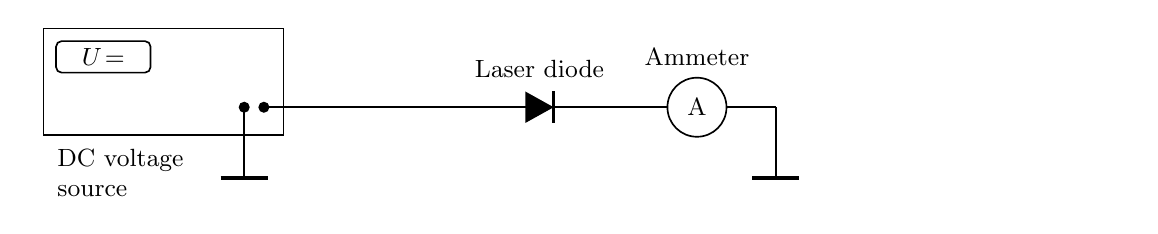
\begin{tikzpicture}[setup]
			\path (-3,0) -- (11,0);
			\pic (src) at (0,0) {instrument={$U\!=$}};
			\node[anchor=north west, align=left] at (-2.75,-0.4) {DC voltage\\source};
			\pic at (src-a) {ground};
			\draw (src-b) -- (6.5,0);
			\pic at (3.5,0) {diode};
			\node[above] at (3.5,0.25) {Laser diode};
			\node[meter] at (5.5,0) {A};
			\node[above] at (5.5,0.4) {Ammeter};
			\pic at (6.5,0) {ground};
		\end{tikzpicture}
		\caption{Current-voltage characteristic.}
		\label{fig:setup_iu}
	\end{subfigure}

	\vspace{0.6cm}
	\begin{subfigure}{\linewidth}
		\centering
		\begin{tikzpicture}[setup]
			\path (-3,0) -- (11,0);
			\pic (gen) at (0,0) {instrument={$I\!=$}};
			\node[anchor=north west, align=left] at (-2.75,-0.4) {Pulse\\generator};
			\pic at (gen-a) {ground};
			\draw (gen-b) -- (5.9,0);
			\draw (0.6,0.15) -- (0.9,0.15) -- (0.9,0.6) -- (1.2,0.6) -- (1.2,0.15) -- (1.5,0.15);
			% voltage measurement at the diode
			\fill (2.2,0) circle (2pt);
			\node[meter] (V) at (2.2,-1.0) {U};
			\draw (2.2,0) -- (V);
			\pic at (V.south) {ground};
			% laser diode on mount with detector
			\pic at (3.6,0) {mount};
			\pic at (3.6,0) {diode};
			\pic at (3.6,0) {emission};
			\draw (4.3,0.8) rectangle (5.5,1.1);
			\node[above] at (4.9,1.1) {Detector};
			\node[meter] at (5.1,0) {A};
			\pic at (5.9,0) {ground};
			% lock-in amplifier
			\pic (lock) at (10.5,0) {instrument={Lock-in}};
			\draw (5.5,0.95) -- (6.8,0.95) -- (6.8,-0.6) -- (10.25,-0.6) -- (lock-a);
			\pic at (lock-b) {ground};
		\end{tikzpicture}
		\caption{Optical power-current characteristic.}
		\label{fig:setup_pi}
	\end{subfigure}

	\vspace{0.6cm}
	\begin{subfigure}{\linewidth}
		\centering
		\begin{tikzpicture}[setup]
			\path (-3,0) -- (11,0);
			\pic (src) at (0,0) {instrument={$I\!=$}};
			\node[anchor=north west, align=left] at (-2.75,-0.4) {DC current\\source};
			\pic at (src-a) {ground};
			\draw (src-b) -- (5.3,0);
			\pic at (3.2,0) {mount};
			\pic at (3.2,0) {diode};
			\pic at (3.2,0) {emission};
			\node[meter] at (4.5,0) {A};
			\pic at (5.3,0) {ground};
			% lens focusing onto the monochromator entrance slit
			\draw (4.0,1.25) ellipse (0.12 and 0.42);
			\draw (4.1,1.6) -- (6.0,1.25) -- (4.1,0.9);
			\draw (6.0,0.6) rectangle (9.2,1.9);
			\node[anchor=south east] at (9.2,0.6) {Monochromator};
			\draw (9.2,1.3) rectangle (10.3,1.9);
			\node at (9.75,1.6) {PMT};
			% computer
			\draw[rounded corners=2pt] (7.9,-1.05) rectangle (9.1,0.05);
			\draw[rounded corners=1pt] (8.05,-0.9) rectangle (8.95,-0.1);
			\draw (8.3,-1.05) -- (8.2,-1.3) -- (8.8,-1.3) -- (8.7,-1.05);
			\draw (7.6,-1.3) rectangle (9.6,-1.85);
			\foreach \x in {7.75,7.85,...,8.45} \draw (\x,-1.42) -- (\x,-1.73);
			\draw (8.9,-1.5) rectangle (9.4,-1.65);
			\draw (9.75,1.3) .. controls (9.9,0.0) and (10.1,-1.4) .. (9.6,-1.55);
		\end{tikzpicture}
		\caption{Spectral measurements.}
		\label{fig:setup_spectral}
	\end{subfigure}
	\caption{Measurement setups for the characterisation of the laser diode. The diode
	is placed on a temperature-controlled mount for the P-I and spectral measurements.
	PMT: photomultiplier tube.}
	\label{fig:setup}
\end{figure}


\section{Measurement and Results}
\label{sec:measurement_and_results}

This report examines different properties of a laser diode. Current-voltage and optical
power-current characteristics were measured with the setups displayed in
\cref{fig:setup_iu} and \cref{fig:setup_pi}, respectively, and are evaluated in
\cref{sec:iu_pi}. The temperature dependence of the threshold current
is examined in \cref{sec:t0}.

The spectrum of the laser diode is analyzed for different driving currents.
Based on its magnitude, the diode behaves either as an LED, see
\cref{sec:spontaneous_emission_spectra} or as a laser diode, see \cref{sec:mode_spectrum}.
Finally, the power density in the active region is estimated in \cref{sec:power_density}.

\subsection{I-U and P-I Characteristics}
\label{sec:iu_pi}

\begin{figure}
	\centering
	\includegraphics{../plots/task1_V_I.pdf}
	\caption{Current-voltage characteristics of the laser diode, in linear (left) and
	logarithmic (right) scaling.}
	\label{fig:task1_V_I}
\end{figure}

\begin{figure}
	\centering
	\includegraphics{../plots/task1_I_P.pdf}
	\caption{Power-current characteristics of the laser diode, in linear (left) and
	logarithmic (right) scaling.}
	\label{fig:task1_I_P}
\end{figure}

\begin{figure}
	\centering
	\includegraphics{../plots/task1_I_eta.pdf}
	\caption{Wall-plug efficiency of the laser diode in logarithmic scaling.}
	\label{fig:task1_I_eta}
\end{figure}

The laser diode's current-voltage characteristic curve was measured at a temperature
of \qty{22}{\degreeCelsius} and is depicted in \cref{fig:task1_V_I}. For low
voltages, the exponential shape of the ideal diode is dominant. For higher
voltages, the linear shape of the series resistance becomes increasingly significant.

To evaluate the contact quality, \cref{eq:schockley_real} is used as a fit
function for currents up to \qty{12}{\milli \ampere}. Above the threshold current,
the gain clamps the quasi-Fermi level splitting and thereby the junction voltage,
which then no longer follows the diode law. The fit yields $R_{\mathrm{s}}
=\qty{10.2(3)}{\ohm}$ and an ideality factor of $n_{\mathrm{id}}=\num{2.02(3)}$.
For currents above \qty{14}{\milli \ampere}, the junction voltage is constant and the
voltage rises only by the drop over the series resistance. A linear fit
$V=V_{0}+R_{\mathrm{s}}I$ was applied, resulting in $R_{\mathrm{s}}=\qty{9.5(1)}{\ohm}$
and $V_{0}=\qty{1.629(1)}{\volt}$. The intercept $V_{0}$ is the clamped junction
voltage, i.e., $eV_{0}=F_{\mathrm{n}}-F_{\mathrm{p}}$. It exceeds the photon energy
$\hbar\omega=\qty{1.594}{\electronvolt}$ of the lasing mode at \qty{778}{\nano\meter}
(\cref{sec:mode_spectrum}), as required by the Bernard-Duraffourg condition
(\cref{sec:bernard_duraffourg}).

The optical power-current characteristics were measured at a temperature of \qty{22}{\degreeCelsius}
and are displayed in \cref{fig:task1_I_P}. For low currents up to $I_{\mathrm{th}}$,
the optical power is nearly zero. As the laser diode is effectively acting as an LED,
the incoherent light is emitted over a large solid angle. Consequently, the
detector only measures a small fraction of the total output power. For currents larger
than $I_{\mathrm{th}}=\qty{12.81(1)}{\milli\ampere}$, the optical power rises
sharply. As the threshold current is reached, all additional current is used
for stimulated emission and a linear response is established, as predicted by \cref{eq:p_i_function}.
Lasing starts and coherent light is emitted in a narrow solid angle. The fit yields
a differential efficiency of $\eta_{\mathrm{d}}=\qty{9.18(2)}{\percent}$. The
wall-plug efficiency is displayed in \cref{fig:task1_I_eta}.

\subsection{Temperature Dependence of the Threshold Current}
\label{sec:t0}

\begin{figure}
	\centering
	\includegraphics{../plots/task2.pdf}
	\caption{Power-current characteristics of the laser diode for different
	temperatures (left) and threshold current as a function of temperature (right).}
	\label{fig:task2}
\end{figure}

The power-current characteristic curves of the laser diode were recorded for
different temperatures, ranging from \qtyrange{14}{50}{\celsius}, see \cref{fig:task2}.
For each curve, the threshold current was determined using a linear fit, similar
to \cref{sec:iu_pi}. The threshold current as a function of temperature can be fitted
using \cref{eq:current_temperature} and yields a characteristic temperature of $T
_{0}=\qty{117(3)}{\kelvin}$.

\subsection{Spontaneous Emission Spectra}
\label{sec:spontaneous_emission_spectra}

\begin{figure}
	\centering
	\includegraphics{../plots/task3.pdf}
	\caption{Emission spectrum of the laser diode at \qty{0.1}{\milli \ampere}
	and \qty{9.9}{\milli \ampere} in semi-logarithmic (left) and linearized (right) representation.}
	\label{fig:task3}
\end{figure}

The spectral response of the laser diode was measured at a low current of \qty{0.1}{\milli \ampere}
and an intermediate current of \qty{9.9}{\milli \ampere}. The curves are
displayed in \cref{fig:task3}. As both currents are below threshold, a
spontaneous emission response is expected. For this purpose, the function $p_{\lambda}$, see
\cref{eq:spontaneous_emission_line_shape} is fitted logarithmically to the line shape
on the high-energy flank. As $E_{\mathrm{g}}$ is tied to the energy $E_{\mathrm{peak}}$
of the measured maximum via the exact position of the maximum of $p_{\lambda}$,
$E_{\mathrm{peak}}= E_{\mathrm{g}}+ (k_{\mathrm{B}}T_{\mathrm{c}}/2)/(1-4k_{\mathrm{B}}T_{\mathrm{c}}/E_{\mathrm{peak}})$,
only $T_{\mathrm{c}}$ and the amplitude are free parameters.

The spectrum at $I=\qty{0.1}{\milli \ampere}$ features a broad line
with a FWHM of \qty{20}{\nano \meter}, indicating pure LED operation. The fit yields
a carrier temperature of $T_{\mathrm{c}}= \qty{268(4)}{\kelvin}$, about \qty{27}{\kelvin}
below room temperature. This temperature is unphysical, as the carriers cannot be
colder than the lattice. A possible cause is the uncalibrated spectral response of
the detection system. The band gap of $E_{\mathrm{g}}= \qty{1.573}{\electronvolt}$
indicates an \ce{AlGaAs} active layer. With the direct band gap
$E_{\mathrm{g}}(x)=\qty{1.42}{\electronvolt}+x\cdot\qty{1.25}{\electronvolt}$ of
$\mathrm{Al}_{x}\mathrm{Ga}_{1-x}\mathrm{As}$ for $x<0.4$
\cite{grundmann_physics_2021}, this corresponds to an
aluminum fraction of $x\approx\num{0.12}$.

The spectrum at \qty{9.9}{\milli\ampere} features a narrower line with a FWHM of
\qty{4.8}{\nano\meter} and a carrier temperature of
$T_{\mathrm{c}}= \qty{222(2)}{\kelvin}$. This is not a physical carrier temperature,
as gain effects influence the emission behavior.

\subsection{Mode Spectrum and Effective Refractive Index}
\label{sec:mode_spectrum}

\begin{figure}
	\centering
	\includegraphics{../plots/task5.pdf}
	\caption{Emission spectrum of the laser diode at \qty{19}{\milli \ampere}, logarithmic
	intensity axis. The curve is cut off at the main mode at about \qty{778}{\nano\meter}
	by the detector saturation.}
	\label{fig:task5}
\end{figure}

The spectral response of the laser diode was measured at
$I=\qty{19}{\milli \ampere}>I_{\mathrm{th}}$ and is displayed in \cref{fig:task5}.
The spectrum features a series of equidistant peaks that are equally spaced by
$\Delta \lambda=\qty{0.250(5)}{\nano \meter}$. Using \cref{eq:laser_spacing}, $\Delta
m = 1$, $\mathrm{d}\bar{n}/\mathrm{d}\lambda \simeq 0$ and the cavity length of
$L=\qty{300}{\micro \meter}$, the effective refractive index is $\bar{n}=\num{4.02(8)}$.
It is close to the refractive index of \ce{GaAs} (\num{3.4})
\cite[Table~1.1]{grundmann_physics_2021}.

\subsection{Power Density in the Active Volume}
\label{sec:power_density}

At \qty{19}{\milli\ampere}, the registered optical power is \qty{0.9}{\milli\watt}.
By estimating the active volume as
\begin{equation}
	L = \qty{300000}{\nano\meter}, \quad w = \qty{5000}{\nano\meter}, \quad d = \qty
	{20}{\nano\meter}, \qquad V=\qty{3e-17}{\meter\cubed},
\end{equation}
the power density can be calculated as
$P_{\mathrm{opt}}/ V = \qty{3e13}{\watt\per\meter\cubed}$.
For comparison, a Ryzen 5800X3D processor has a default \ac{tdp} of 
\qty{105}{\watt} and a compute die size of \qty{74}{\milli\meter\squared}. By estimating 
a chip thickness of \qty{775}{\micro\meter}, this corresponds to a power density of approximately
\qty{2e9}{\watt \per \meter \cubed} \cite{noauthor_amd_nodate}. 